\documentclass[tikz,border=10pt]{standalone}
\usepackage{amsmath}
\usepackage{tikz}
\usetikzlibrary{arrows.meta, positioning, calc, shapes.geometric}

\begin{document}
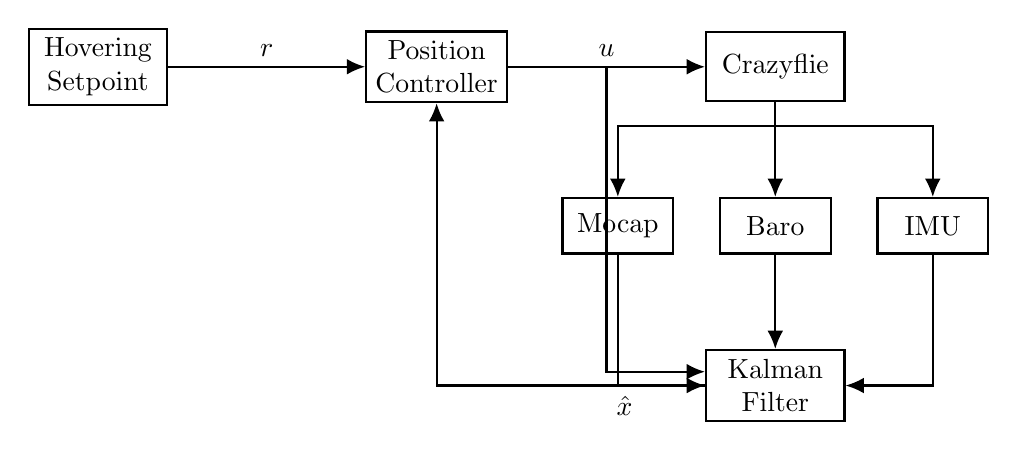
\begin{tikzpicture}[
  block/.style = {draw, thick, minimum height=2.5em, minimum width=5em, align=center},
  smallblock/.style = {draw, thick, minimum height=2em, minimum width=4em, align=center},
  arrow/.style = {thick, -{Latex[width=2mm]}},
  node distance=2.2cm and 2.2cm
]

  % Setpoint
  \node[block] (setpoint) {Hovering\\Setpoint};

  % Controller
  \node[block, right=2.5cm of setpoint] (controller) {Position\\Controller};

  % Plant
  \node[block, right=2.5cm of controller] (plant) {Crazyflie};

  % Three sensors below plant
  \node[smallblock, below=1.2cm of plant, xshift=-2cm] (mocap) {Mocap};
  \node[smallblock, below=1.2cm of plant] (baro) {Baro};
  \node[smallblock, below=1.2cm of plant, xshift=2cm] (imu) {IMU};

  % Observer
  \node[block, below=1.2cm of baro] (observer) {Kalman\\Filter};

  % Reference signal: setpoint -> controller
  \draw[arrow] (setpoint.east) -- node[above] {$r$} (controller.west);

  % Control signal: controller -> plant
  \draw[arrow] (controller.east) -- node[above] {$u$} (plant.west);

  % Control branch to observer
  \coordinate (usplit) at ($(controller.east)!0.5!(plant.west)$);
  \coordinate[above=0.5em of observer.west] (observer_uin);
  \draw[arrow] (usplit) |- (observer_uin);

  % Measurements: plant -> sensors
  \draw[arrow] (plant.south) -- ++(0,-0.3) -| (mocap.north);
  \draw[arrow] (plant.south) -- (baro.north);
  \draw[arrow] (plant.south) -- ++(0,-0.3) -| (imu.north);

  % Sensors -> observer
  \draw[arrow] (mocap.south) |- (observer.west);
  \draw[arrow] (baro.south) -- (observer.north);
  \draw[arrow] (imu.south) |- (observer.east);

  % State estimate: observer -> controller
  \draw[arrow] (observer.west) -| node[pos=0.15, below] {$\hat{x}$} (controller.south);

\end{tikzpicture}
\end{document}
